\documentclass[a4paper]{article}
\usepackage[T1]{fontenc}
\usepackage[utf8]{inputenc}
\usepackage[english]{babel}
\usepackage{amsmath}
\usepackage{amsfonts}
\usepackage{amssymb}
\usepackage{tikz}
\usepackage{resizegather} \addtolength{\jot}{4pt}
\usepackage{microtype}

\renewcommand{\vec}[1]{\mathbf{#1}}
\DeclareMathOperator*{\argmin}{\arg\!\min}
\DeclareMathOperator*{\argmax}{\arg\!\max}
\DeclareMathOperator*{\esssup}{ess\sup}
\DeclareMathOperator{\sgn}{sgn}
\DeclareMathOperator{\diver}{div}
\DeclareMathOperator{\supp}{supp}
\newcommand{\dx}{\, dx \,}
\newcommand{\dy}{\, dy \,}
\newcommand{\dxy}{\, dx \:\! dy \,}
\newcommand{\dvecx}{\, d\vec{x} \,}
\newcommand{\dsigma}{\, d\sigma \,}
\newcommand{\area}[1]{\left\lvert #1 \right\rvert}
\newcommand{\abs}[1]{\left\lvert #1 \right\rvert}
\newcommand{\seminorm}[1]{\left\lvert #1 \right\rvert}
\newcommand{\norm}[1]{\left\lVert #1 \right\rVert}
\newcommand{\dpair}[1]{\left\langle #1 \right\rangle}
\newcommand{\R}{\mathbb{R}}
\newcommand{\N}{\mathbb{N}}
\newcommand{\Pone}{\mathbb{P}_1}

\title{\huge{Advanced Discretization Techniques \\ Homework 6}}
\author{\Large{Bruno Degli Esposti, Xingyu Xu}}
\date{November 26th - December 3rd, 2019}

\begin{document}

\maketitle

\section*{Exercise 13: Instability of $(\mathcal{P}_1)^2\text{-}(\mathcal{P}_1)$ for Stokes}
\begin{description}
\item[a)] One way to construct such a function $p_h \in S_0^1$ is as follows:

	\begin{figure}[h]
	\centering
	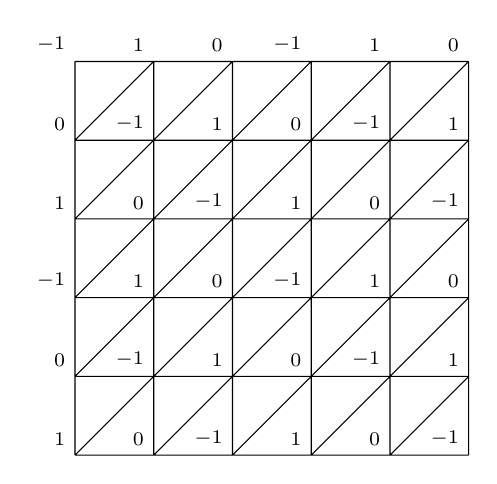
\begin{tikzpicture}
		\draw
			(0, 0) grid[step=1cm] (5, 5)
			(0, 4) -- (1, 5)
			(0, 3) -- (2, 5)
			(0, 2) -- (3, 5)
			(0, 1) -- (4, 5)
			(0, 0) -- (5, 5)
			(1, 0) -- (5, 4)
			(2, 0) -- (5, 3)
			(3, 0) -- (5, 2)
			(4, 0) -- (5, 1)
		;
		\path[above left]
		\foreach \y in {0, 3} {
			\foreach[count=\x] \v in {1,0,-1,1,0,-1} {
				(\x-1, \y) node {$\scriptstyle\v$}
			}
		}
		\foreach \p/\v in {
			{0, 2}/-1, {1, 2}/1, {2, 2}/0, {3, 2}/-1, {4, 2}/1, {5, 2}/0,
			{0, 1}/0, {1, 1}/-1, {2, 1}/1, {3, 1}/0,	{4, 1}/-1, {5, 1}/1,
			{0, 5}/-1, {1, 5}/1, {2, 5}/0, {3, 5}/-1, {4, 5}/1, {5, 5}/0,
			{0, 4}/0, {1, 4}/-1, {2, 4}/1, {3, 4}/0, {4, 4}/-1, {5, 4}/1
		} {
			(\p) node {$\scriptstyle\v$}
		};
	\end{tikzpicture}
	\end{figure}
	
	For any $T \in \mathcal{T}_h$, it's clear from the picture that the values
	of $p_h$ at the three vertices $a_1,a_2,a_3$ of $T$ are always a permutation
	of $\{0,1,-1\}$. Without loss of generality, we can assume that
	$p_h(a_1) = 0, p_h(a_2) = 1, p_h(a_3) = -1$.
	Since $p_h$ is an affine function when restricted to $T$, we get that
	\[
	p_h(\lambda a_i + (1-\lambda) a_j) = \lambda p_h(a_i) + (1-\lambda) p_h(a_j)
	\]
	holds for all $i,j \in \{1,2,3\}$ and all $\lambda \in [0,1]$.
	Then, by the midpoint rule (which is exact for affine functions), it follows that
	\begin{gather*}
	\int_T p_h(x) \dx
	= \frac{\area{T}}{3} \left(
		  p_h \left( \frac{1}{2} a_1 + \frac{1}{2} a_2 \right)
		+ p_h \left( \frac{1}{2} a_2 + \frac{1}{2} a_3 \right)
		+ p_h \left( \frac{1}{2} a_3 + \frac{1}{2} a_1 \right) \right) \\
	= \frac{\area{T}}{3} \left(
		  \frac{1}{2} p_h(a_1) + \frac{1}{2} p_h(a_2)
		+ \frac{1}{2} p_h(a_2) + \frac{1}{2} p_h(a_3)
		+ \frac{1}{2} p_h(a_3) + \frac{1}{2} p_h(a_1) \right) \\
	= \frac{\area{T}}{3} \left(
		  \frac{0}{2}  + \frac{1}{2}
		+ \frac{1}{2}  + \frac{-1}{2}
		+ \frac{-1}{2} + \frac{0}{2} \right)
	= \frac{\area{T}}{3} \left( \frac{2-2}{2} \right)
	= 0.
	\end{gather*}
	This proves that $p_h \in L_0^2$ (the integral over $\Omega$ can be split
	as the sum of the integrals over $T \in \mathcal{T}_h$,
	and square-integrability comes from the fact that
	$\bar{\Omega}$ is a compact set). By construction, $p_h \in S_0^1$.
	Hence, $p_h \in X_h$, as requested.
\item[b)] For the Stokes problem, we have that $b_h \colon M_h \times X_h \to \R$
	is defined as
	\[
	b_h(\vec{v}_h,p_h) = -\int_\Omega p_h \diver(\vec{v}_h) \dx.
	\]
	As usual, we then define the operator $B_h \colon M_h \to X_h^*$ so that
	\[
	b_h(\vec{v}_h,p_h) = \dpair{B_h \vec{v}_h,p_h} = \dpair{\vec{v}_h, B_h^T p_h}.
	\]
	As explained in Knabner-Angermann (8.42, p.\ 399,400), $\ker(B_h^T) \neq \{0\}$
	is enough to ensure that the inf-sup conditions do not hold.
	We will now prove that $p_h \in \ker(B_h^T)$ using the fact that all
	functions in $(\mathcal{P}_1)^2$ have elementwise constant divergence
	(that's what we get when we derive a polynomial of degree at most 1).
	For any $\vec{v}_h \in M_h$,
	\begin{align*}
	\dpair{\vec{v}_h, B_h^T p_h}
&	= -\int_\Omega p_h \diver(\vec{v}_h) \dx
	= -\sum_{T \in \mathcal{T}_h} \int_T p_h \diver(\vec{v}_h) \dx \\
&	= -\sum_{T \in \mathcal{T}_h} \diver(\vec{v}_h) \big{|}_T \int_T p_h \dx
	\stackrel{a)}{=} -\sum_{T \in \mathcal{T}_h} \diver(\vec{v}_h) \big{|}_T \; 0 \dx
	= 0.
	\end{align*}
	This implies that $B_h^T p_h = 0$ and $p_h \in \ker(B_h^T)$, as required. $\square$
\end{description}

\section*{Exercise 14: A stable element - Fortin's trick}
\begin{description}
\item[a)] The subspace $S_{0,0}^1$ of $H_0^1(\Omega)$ is still a Hilbert space
	with respect to the same scalar product, because it's finite dimensional.
	The bilinear form $a_h$ is equal to said scalar product, so it's continuous
	by Cauchy-Schwarz's inequality, and coercive by definition ($\alpha = 1$).
	The inclusion $S_{0,0}^1 \subset H_0^1(\Omega)$ induces the opposite
	inclusion for the dual spaces, so $v$ (as an element of $(H_0^1(\Omega))^*$,
	by Riesz's isometry) is also an element of $(S_{0,0}^1)^*$.
	Then, by Lax-Milgram's lemma,
	\[
	\exists! \; \pi_h^0v \in S_{0,0}^1 \; \text{ such that} \;\;
	a_h(\pi_h^0v, w_h) = \dpair{v, w_h}_1 \text{ for all } w_h \in S_{0,0}^1
	\]
	and we get the stability estimate
	\[
	\norm{\pi_h^0v}_1
	\leq \frac{\norm{v}_{(S_{0,0}^1)^*}}{\alpha}
	\leq \frac{\norm{v}_{(H_0^1(\Omega))^*}}{\alpha}
	= \frac{\norm{v}_1}{\alpha}
	= \norm{v}_1.
	\]
	This is exactly what we wanted to prove.
\item[b)] By equation (A) we get that $a_h(w_h,\pi^0_hv-v)=0$,
	and by equation (B) we get that $a_h(u,\pi^0_hv-v)=(f,\pi^0_hv-v)_0$.
	Since we have assumed here that $f=\pi^0_hv-v$,
	it is now clear by linearity that $a_h(u-w_h,\pi^0_hv-v)=\norm{\pi_h^0v-v}_0^2$.
\item[c)] Since $\Omega \subset \R^2$, $H^2$-regularity of $u$ is enough
	for $I_h u$ to be well-defined ($I_h$ is the Lagrange interpolation operator),
	with an interpolation error estimate of $\norm{u-I_h u}_1 \leq C_I h \norm{u}_2$.
	If we now choose $w_h = I_h u$ in the result of point b), we get that
	\begin{align*}
	\norm{\pi_h^0v-v}_0^2
&	= a_h(u-I_h u,\pi_h^0v-v)
	= \dpair{u-I_h u,\pi_h^0v-v}_1 \\
&	\leq \norm{u-I_h u}_1 \norm{\pi_h^0v-v}_1
	\leq C_I h \norm{u}_2 \norm{\pi_h^0v-v}_1 \\
&	\leq C_I C h \norm{f}_0 \norm{\pi_h^0v-v}_1
	= C_I C h \norm{\pi_h^0v-v}_0 \norm{\pi_h^0v-v}_1.
	\end{align*}
	All that's left to do now is to divide by $\norm{\pi_h^0v-v}_0$.
\item[d)] By the triangle inequality and the results of points a) and c),
	we get that
	\[
	\norm{\pi_h^0v-v}_0
	\leq C h \norm{\pi_h^0v-v}_1
	\leq C h \norm{\pi_h^0v}_1 + C h \norm{v}_1
	\leq 2C h \norm{v}_1.
	\]
\item[e)] By the definition of $B_3$, we need to find a constant $C_T$ for each
	$T \in \mathcal{T}_h$ such that
	\[
	\int_T v \dx
	= \int_T \pi_h^1v \dx
	= \int_T C_T \, \varphi_{T,1} \varphi_{T,2} \varphi_{T,3} \dx.
	\]
	Solving for $C_T$ gives
	\[
	C_T = \left( \int_T v \dx \right)
	      \left( \int_T \varphi_{T,1} \varphi_{T,2} \varphi_{T,3} \dx \right)^{-1}.
	\]
	First of all, we need to make sure that we are not dividing by 0.
	Let $\hat{T}$ be the reference element in $\R^2$. Then, by the change
	of variables formula,
	\begin{gather*}
	\int_T \varphi_{T,1}(\vec{x}) \varphi_{T,2}(\vec{x})
	       \varphi_{T,3}(\vec{x}) \, d\vec{x} \,
	= \int_{\hat{T}} xy(1-x-y) \, 2 \area{T} \! \dxy \\
	= 2 \area{T} \int_0^1 \int_0^{1-x} xy(1-x-y) \dy \dx
	= \frac{2\area{T}}{120}
	= \frac{\area{T}}{60} \neq 0.
	\end{gather*}
	Next, in order to conclude that $\pi_h^1$ is well-defined, we need to
	prove that a function $\pi_h^1v$ defined on every element $T$ as
	\[
	\frac{60}{\area{T}} \left( \int_T v \dx \right)
	\varphi_{T,1} \varphi_{T,2} \varphi_{T,3}
	\]
	belongs to $H_0^1(\Omega)$. This means that we can't have discontinuities
	on any edge of the triangulation. For any edge $e$, let $T_1$ and $T_2$ be
	the two elements in $\mathcal{T}_h$ such that $e = \partial T_1 \cap \partial T_2$.
	Let $a_i, a_j$ be the vertices in $T_1, T_2$ opposite to $e$
	($i$ and $j$ are in local numbering notation).
	Then, for each $x \in e$,
	\begin{align*}
	\frac{60}{\area{T_1}} \left( \int_{T_1} v \dx \right)
	\varphi_{T_1,1}(x) \varphi_{T_1,2}(x) \varphi_{T_1,3}(x) &= 0 \\
	\frac{60}{\area{T_2}} \left( \int_{T_2} v \dx \right)
	\varphi_{T_2,1}(x) \varphi_{T_2,2}(x) \varphi_{T_2,3}(x) &= 0,
	\end{align*}
	because $\varphi_{T_1,i}(x) = 0 = \varphi_{T_2,j}(x)$.
	Hence, $\pi_h^1v$ vanishes on the boundary of every element.
	This not only ensures continuity (so that $\pi_h^1v \in H^1(\Omega)$),
	but also that $\pi_h^1v$ has 0 trace on $\partial\Omega$, as required.
\item[f)] By Jensen's inequality and the change of variables formula we get that
	\begin{align*}
	\norm{\pi_h^1v}_{0,T}^2
&	= 60^2 \left( \frac{1}{\area{T}} \int_{T} v \dx \right)^2
		\int_T \big( \varphi_{T,1}(x) \varphi_{T,2}(x) \varphi_{T,3}(x) \big)^2 \dx \\
&	\leq \frac{60^2}{\area{T}} \left( \int_{T} v^2 \dx \right)
		\int_T \big( \varphi_{T,1}(x) \varphi_{T,2}(x) \varphi_{T,3}(x) \big)^2 \dx \\
&	= \frac{60^2}{\area{T}} \left( \int_{T} v^2 \dx \right)
		2 \area{T} \int_{\hat{T}} \big( \varphi_{T,1}(\hat{x})
		\varphi_{T,2}(\hat{x}) \varphi_{T,3}(\hat{x}) \big)^2 \, d\hat{x} \, \\
&	= \frac{60^2}{\area{T}} \left( \int_{T} v^2 \dx \right) \frac{2\area{T}}{5040}
	= \frac{10}{7} \norm{v}_{0,T}^2
	= C \norm{v}_{0,T}^2.
	\end{align*}
	The rest of the proof is straightforward:
	\[
	\norm{\pi_h^1v}_0^2
	= \sum_{T \in \mathcal{T}_h} \norm{\pi_h^1v}_{0,T}^2
	\leq \sum_{T \in \mathcal{T}_h} C \norm{v}_{0,T}^2
	= C \sum_{T \in \mathcal{T}_h} \norm{v}_{0,T}^2
	= C \norm{v}_0^2
	\]
	and then we take the square root on both sides.
\item[g)] We begin with integration by parts:
	\begin{align*}
	b(v-\Pi_h v, q_h)
	= &- \int_\Omega q_h \diver(v-\pi_h^0v-\pi_h^1(v-\pi_h^0v)) \dx \\
	= &- \int_{\partial\Omega} q_h (v-\pi_h^0v-\pi_h^1(v-\pi_h^0v)) \cdot n \dsigma \\
	  &+ \int_\Omega \nabla q_h \cdot (v-\pi_h^0v-\pi_h^1(v-\pi_h^0v)) \dx.
	\end{align*}
	The boundary term vanishes, because the functions $v$, $\pi_h^0v$
	and $\pi_h^1(v-\pi_h^0v)$ are all in $H_0^1(\Omega)^2$.
	As for the other term, we will use point e) and the fact that
	$\nabla q_h$ is elementwise constant (it's the gradient of a polynomial
	of degree at most 1) to show that it vanishes, too:
	\begin{gather*}
	\int_\Omega \nabla q_h \cdot (v-\pi_h^0v-\pi_h^1(v-\pi_h^0v)) \dx
	= \sum_{T \in \mathcal{T}_h} \int_T \nabla q_h
		\cdot (v-\pi_h^0v-\pi_h^1(v-\pi_h^0v)) \dx \\
	= \sum_{T \in \mathcal{T}_h} \nabla q_h
		\cdot \int_T (v-\pi_h^0v)-\pi_h^1(v-\pi_h^0v) \dx
	\stackrel{e)}{=} \sum_{T \in \mathcal{T}_h} \nabla q_h
		\cdot (0,0)^T \dx
	= 0.
	\end{gather*}
\item[h)] By Lemma 4.5.3 in Brenner and Scott's \emph{The Mathematical Theory of FEM},
	the following global inverse estimate holds:
	\[
	\norm{\pi_h^1(v-\pi_h^0v)}_1 \leq C_\text{inv} h^{-1} \norm{\pi_h^1(v-\pi_h^0v)}_0.
	\]
	Now we can combine all the results from the previous points to get that
	\begin{align*}
	\norm{\Pi_h v}_1
&	= \norm{\pi_h^0 v + \pi_h^1(v-\pi_h^0v)}_1
	\leq \norm{\pi_h^0 v}_1 + \norm{\pi_h^1(v-\pi_h^0v)}_1 \\
&	\overset{a)}{\leq} \norm{v}_1 + \norm{\pi_h^1(v-\pi_h^0v)}_1
	\leq \norm{v}_1 + C_\text{inv} h^{-1} \norm{\pi_h^1(v-\pi_h^0v)}_0 \\
&	\overset{f)}{\leq} \norm{v}_1 + C_\text{inv} h^{-1} C_\text{f} \norm{v-\pi_h^0v}_0
	\overset{d)}{\leq} \norm{v}_1 + C_\text{inv} h^{-1} C_\text{f} C_\text{d} h \norm{v}_1 \\
&	= (1 + C_\text{inv} C_\text{f} C_\text{d}) \norm{v}_1
	= C \norm{v}_1. \quad \square
	\end{align*}
\end{description}

\end{document}





























